\section{Problem 1a: High Gain Amplifier}
\label{sec:A2P1}

\subsection{Ideal Biasing Network}
In accordance with the text delivered in the \hyperref[sec:Foreword]{Foreword}
the ideal design is given below. I have simulated the scattering parameters
according the schematic (biasing) shown in figure
\ref{fig:A2P1IdealSchematic}.

\begin{figure}[H]
    \centering
    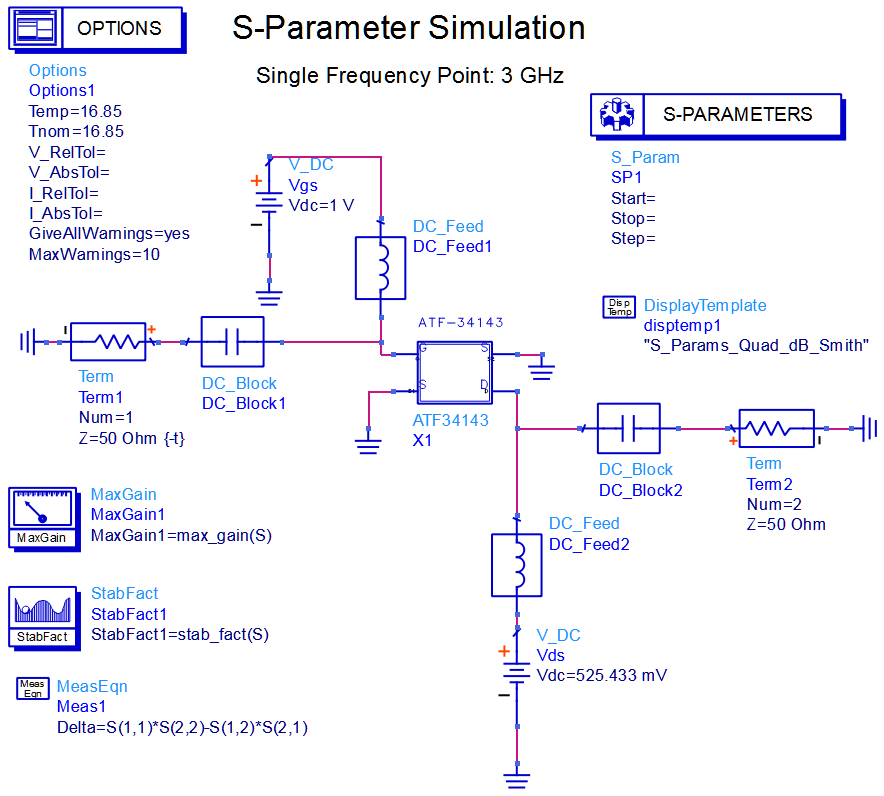
\includegraphics[width=0.8\linewidth]{Images/A2P1IdealSchematic.png}
    \caption{Schematic of the biasing network for the high-gain amplifier}
    \label{fig:A2P1IdealSchematic}
\end{figure}

The results of simulating this biasing network are given in figure
\ref{fig:A2P1IdealBiasingResults}.

\begin{figure}[H]
    \centering
    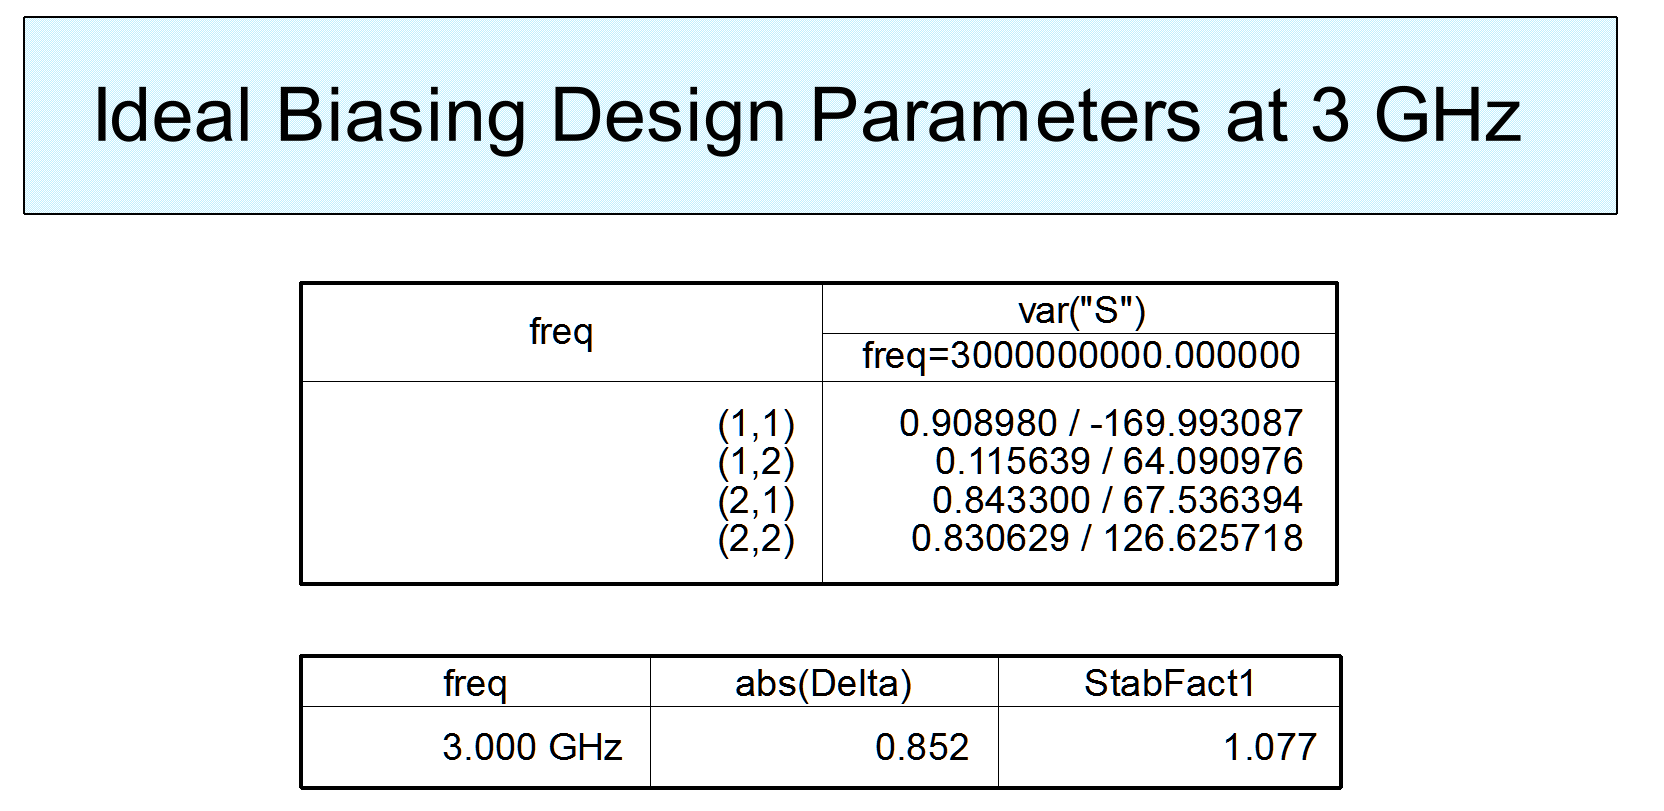
\includegraphics[width=0.8\linewidth]{Images/A2P1IdealBiasingResults}
    \caption{Results of simulating the biasing network shown in figure
    \ref{fig:A2P1IdealSchematic}}
    \label{fig:A2P1IdealBiasingResults}
\end{figure}

\subsection{Physical Biasing Network}
If I replace the DC feeds (ideal inductors) and DC blocks (ideal capacitors)
with the following values I obtain the following schematic and results:

\begin{figure}[H]
    \centering
    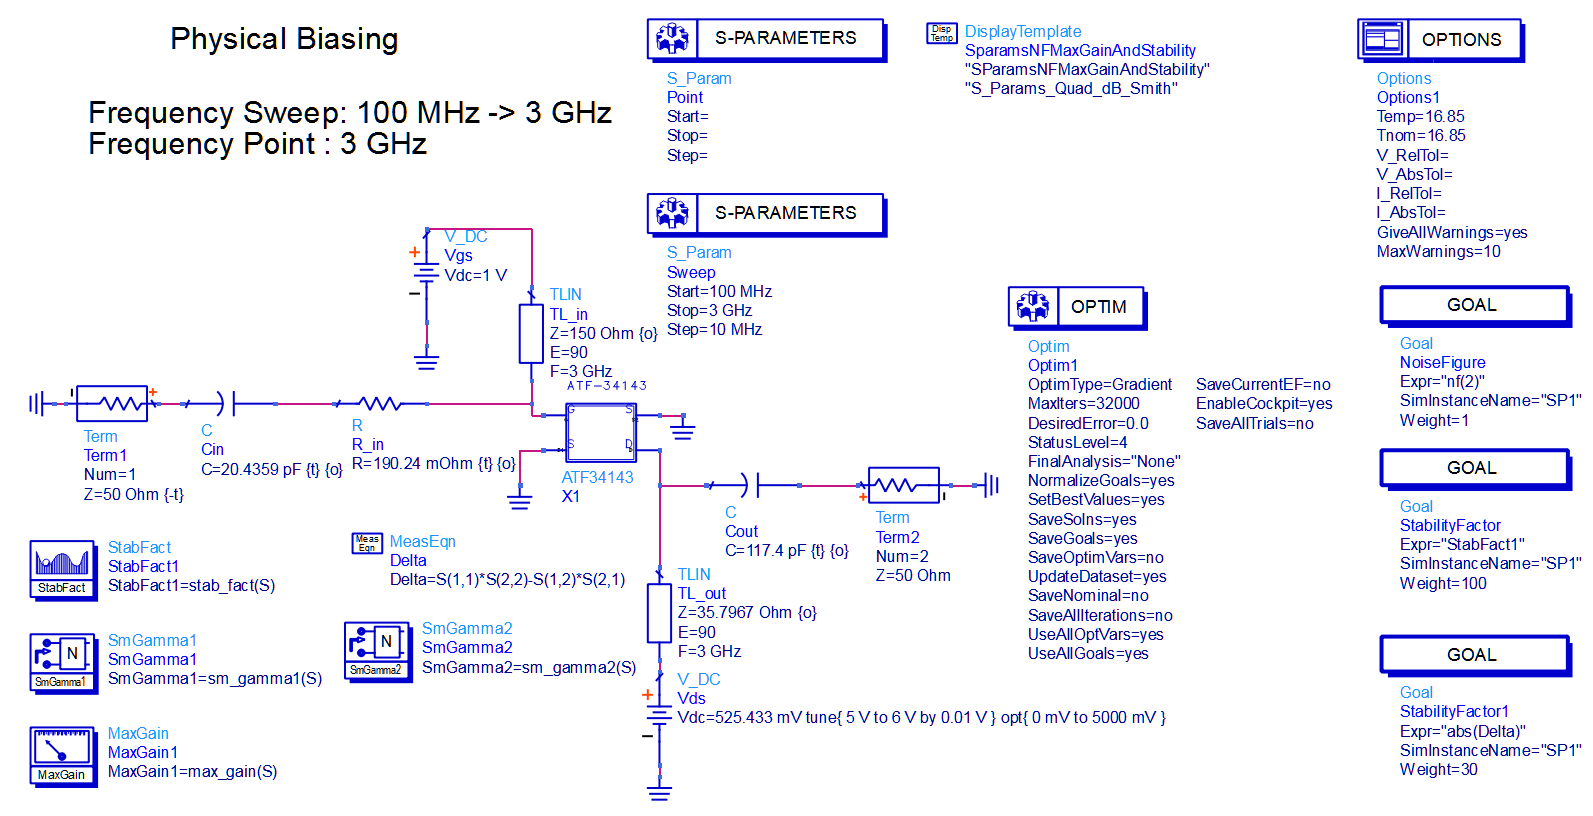
\includegraphics[width=0.8\linewidth]{Images/A2P1PhysicalSchematic.png}
    \caption{High-gain amplifier biasing network using real components}
    \label{fig:A2P1PhysicalSchematic}
\end{figure}

\begin{figure}[H]
    \centering
    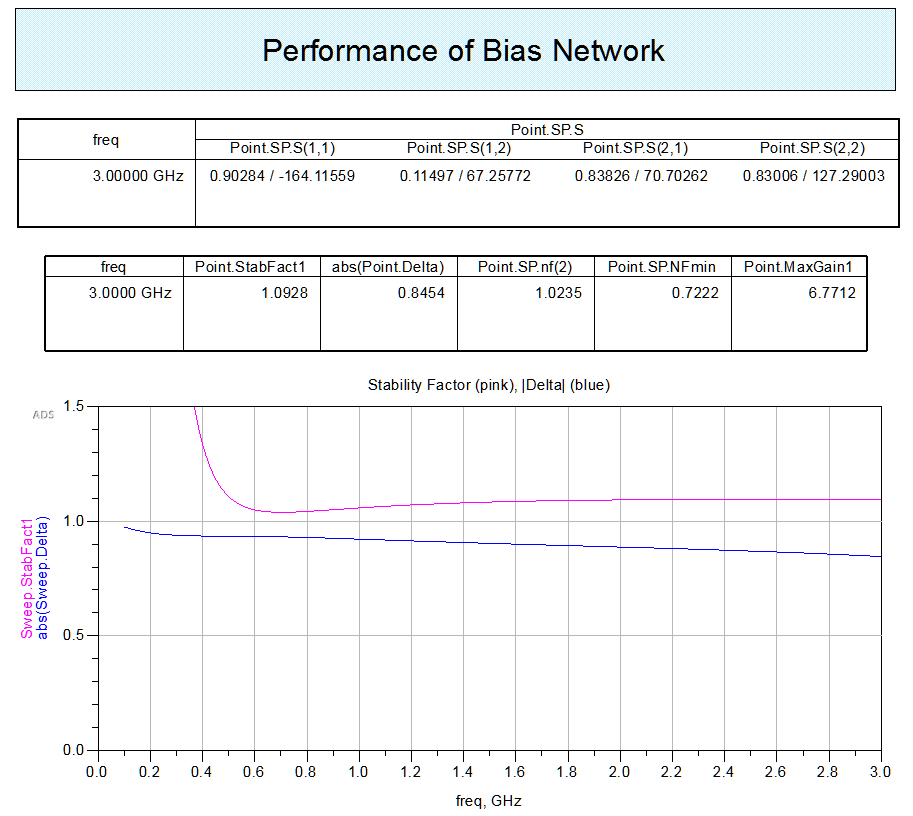
\includegraphics[width=0.8\linewidth]{Images/A2P1PhysicalBiasingResults.png}
    \caption{Real-component biasing results for the high-gain amplifier.}
    \label{fig:A2P1PhysicalBiasingResults}
\end{figure}

In the appendix I derive the relationship between the physical network and the
ideal network. There, I also include the code that I have used to relate the scattering
parameters obtained by simulating the ideal biasing to that of the network
comprising the physical components. Note that while it is known that short
transmission lines of low impedance behave like inductors, the transmission
lines used to couple $V_{gs}$ and $V_{ds}$ to the amplifier suffice even though
they are not sufficiently short or sufficiently low in impedance to qualify as
inductors. This was a design choice. Below, I include a table for easy
comparison that relates the values of $S_{11}, S_{12}, S_{21}, S_{22}$ obtained
using a simulation with the values obtained using MATLAB.

\begin{center}
    \begin{tabular}{|c|c|c|}
        \hline Scattering Parameter & ADS Value & ``Hand-calculated'' MATLAB values \\
        \hline $S_{11}$ & .90284 \phase{-164.12 \degree} & .90283
        \phase{-164.12 \degree} \\
        \hline $S_{12}$ & .11497 \phase{67.257 \degree} & .11495 \phase{67.257
    \degree}\\
        \hline $S_{21}$ & .83826 \phase{70.703 \degree} & .83838 \phase{70.702
\degree} \\
        \hline $S_{22}$ & .83006 \phase{127.29 \degree}  & .83003 \phase{127.29
        \degree} \\ \hline
    \end{tabular}
\end{center}

Note that the stability of the transistor at the design frequency was also
assessed using ADS. ``Hand calculations'' of the Rollett stability factor as
well as the determinant of the scattering parameter matrix are given in the
appendix. They do not differ significantly from the ADS values (they are within
numerical error: a part in ten thousand) so they have not been included here.

Since the transistor is unconditionally stable at the design frequency ($K >1$
and $|\Delta|<1$) no shunting resistor will be used to stabilize the device.

\subsection{Full Design: A High-Gain Amplifier}

The last thing to do is insert a matching network that accomplishes the goal of
the design: To deliver more power to the load. According to the design
requirements, the matching network must be such that $G_{T_{max}} - G_t \le 1$.
A feature that the customer is requiring the lowest noise figure as is possible
given a particular transducer gain, $G_t$. No lower bound is placed on the
values of $G_{T_{max}}$, so given that there is typically a trade-off between
transducer gain and noise figure it makes sense to reduce the noise figure to
something sufficiently low while keeping the gain sufficiently high. Granted,
the \SI{6}{\deci\bel} of transducer gain provided by this design is not great.
However, the noise figure is very low ($< \SI{1}{\deci\bel}$) which was
prioritized over the forward gain.

The design of the amplifier is given below in figure
\ref{fig:A2P1AmplifierSchematic}. The results are given below in figures
\ref{fig:A2P1AmplifierDesignFrequencyEfficacy},\ref{fig:A2P1AmplifierFrequencySweepStability},\ref{fig:A2P1AmplifierFOM}.

Note the addition of the series resistor at the input to the gate of the
amplifier. This was used to stabilize the transistor over the specified $
\SI{100}{\mega\hertz} \rightarrow \SI{3}{\giga\hertz}$ bandwidth.

\begin{figure}[H]
    \centering
    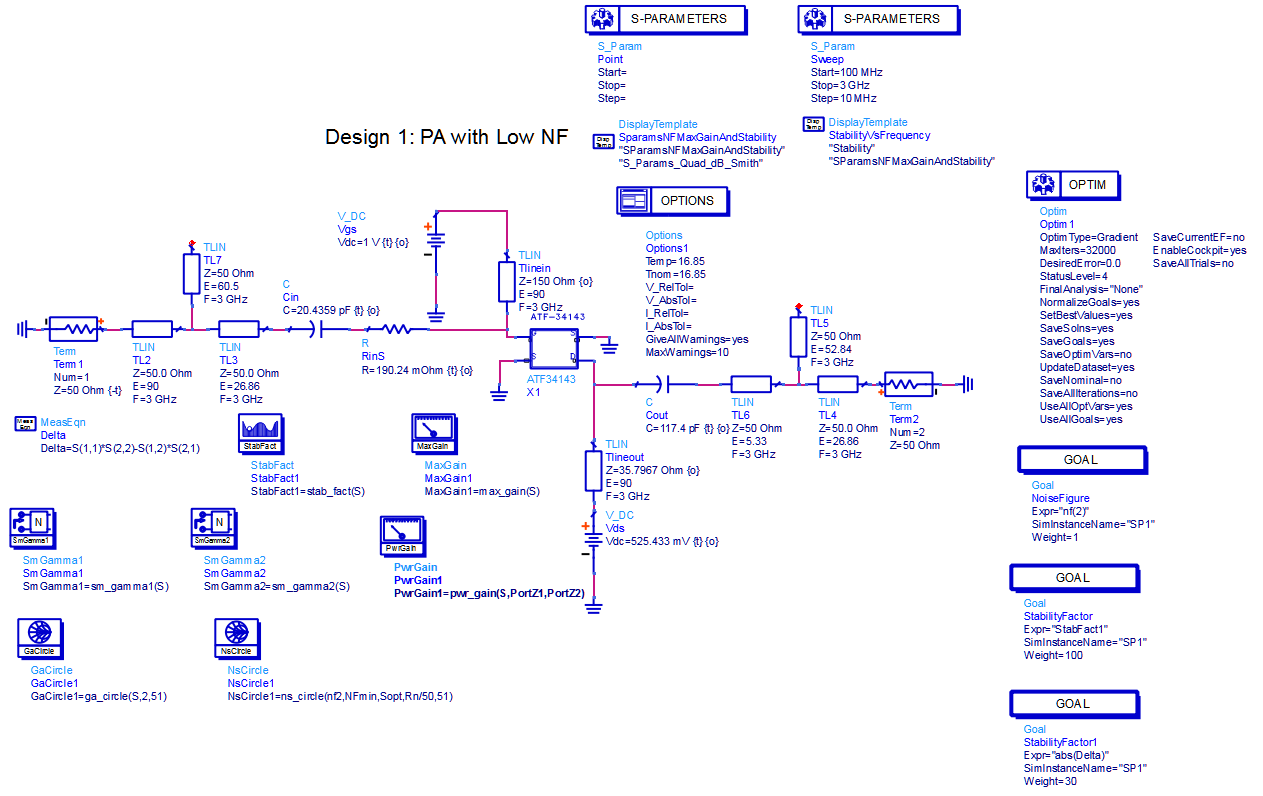
\includegraphics[width=0.8\linewidth]{Images/A2P1AmplifierSchematic.png}
    \caption{Schematic of the high gain amplifier}
    \label{fig:A2P1AmplifierSchematic}
\end{figure}

\begin{figure}[H]
    \centering
    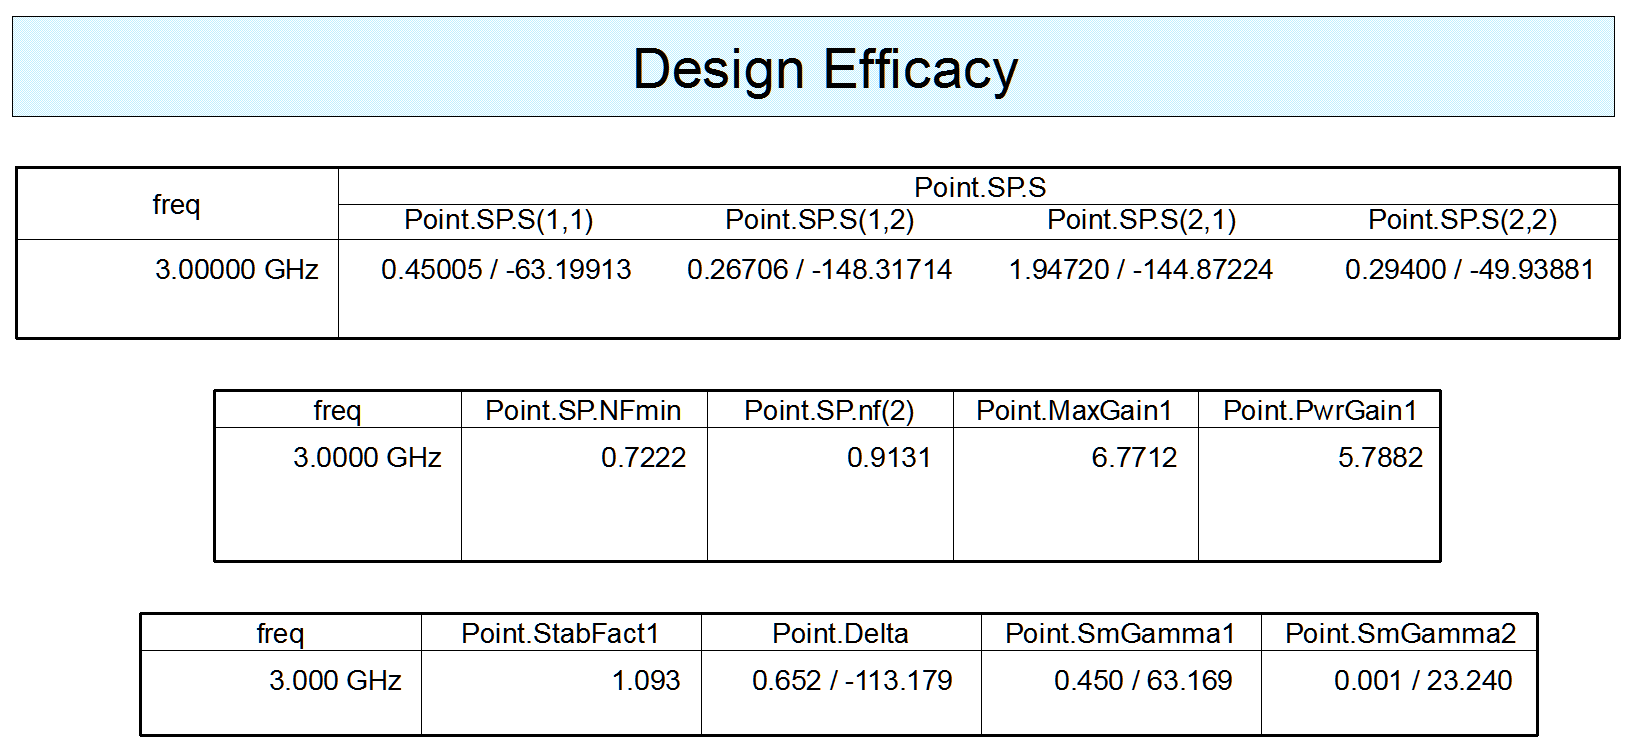
\includegraphics[width=0.8\linewidth]{Images/A2P1AmplifierDesignFrequencyEfficacy.png}
    \caption{Efficacy of the amplifier at the design frequency}
    \label{fig:A2P1AmplifierDesignFrequencyEfficacy}
\end{figure}

\begin{figure}[H]
    \centering
    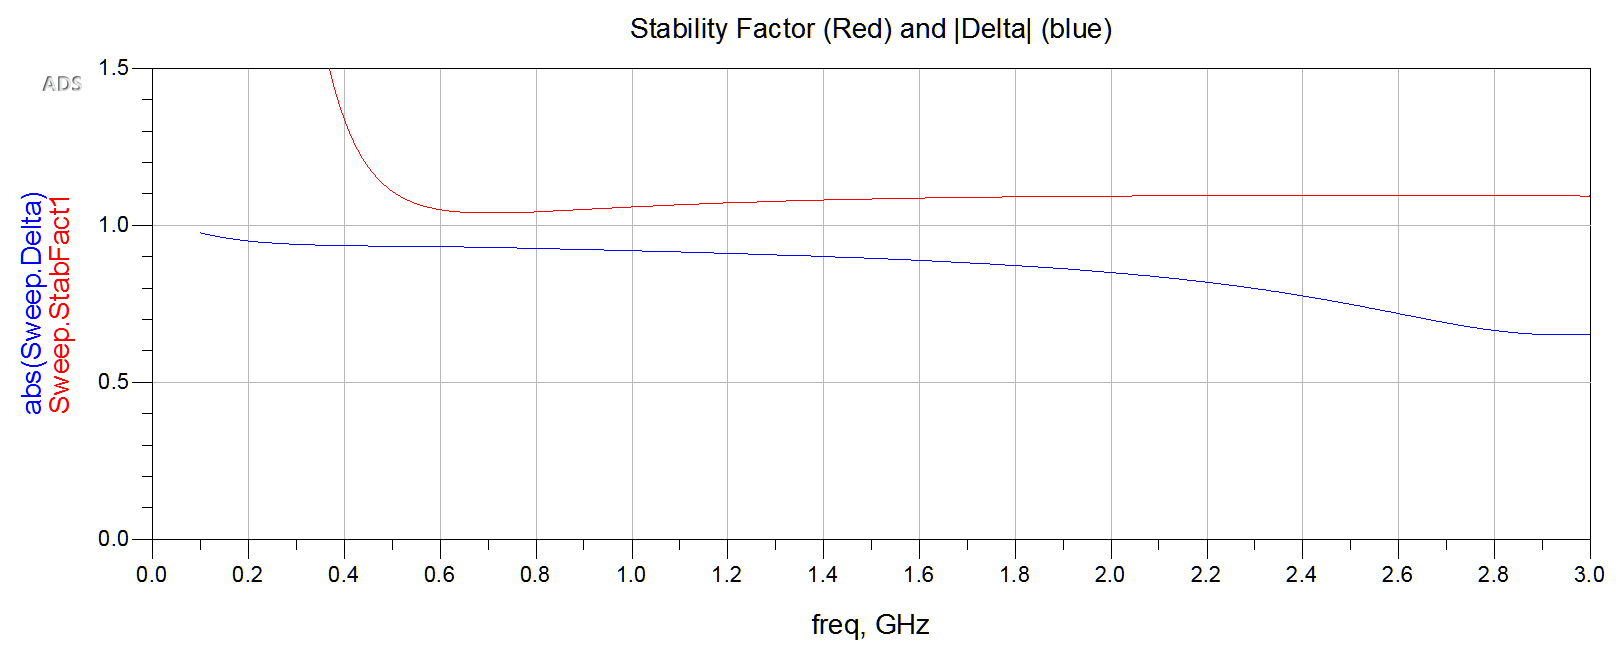
\includegraphics[width=0.8\linewidth]{Images/A2P1AmplifierFrequencySweepStability.png}
    \caption{Stability of the amplifier over the required bandwidth}
    \label{fig:A2P1AmplifierFrequencySweepStability}
\end{figure}

\begin{figure}[H]
    \centering
    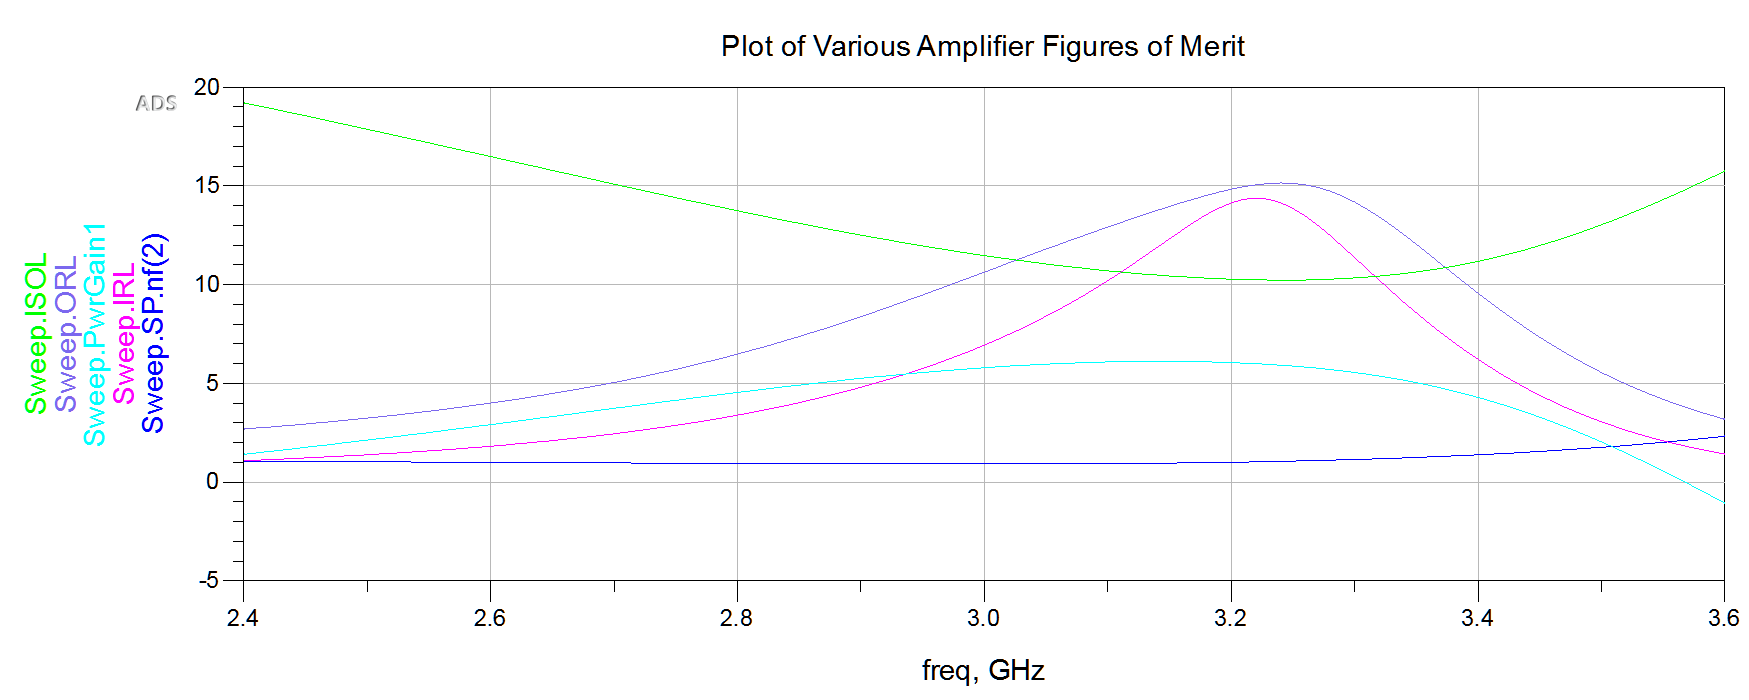
\includegraphics[width=0.8\linewidth]{Images/A2P1AmplifierFOM.png}
    \caption{Plot of various figures of merit of the amplifier including:
    Isolation (green), output return loss (purple), power gain (teal), input
return loss (pink) and noise figure (blue)}
    \label{fig:A2P1AmplifierFOM}
\end{figure}

A few notes regarding the design of the amplifier. It has already been noted
that the gain is not as high as could be attained with this transistor ($\approx
\SI{18}{\deci\bel}$) but noise figure was prioritized. Furthermore, you may
notice that terminal 1 is not matched to the rest of the amplifier circuit. This
was intentional. Introducing mismatch allowed the gain to be reduced which
reduced the noise figure even more than it had been. Note that the gain is still
within the specified distance from $G_{t_{max}}$ in that $G_{T_{max}} - G_T
\approx \SI{.993}{\deci\bel}$.
